\documentclass{article}
\usepackage{graphicx} % Required for inserting images
\usepackage{listings}
\usepackage{float}
\usepackage{tikz}
\lstset{
    inputencoding = utf8,  % Input encoding
    extendedchars = true,  % Extended ASCII
    literate      =        % Support additional characters
      {á}{{\'a}}1  {é}{{\'e}}1  {í}{{\'i}}1 {ó}{{\'o}}1  {ú}{{\'u}}1
      {Á}{{\'A}}1  {É}{{\'E}}1  {Í}{{\'I}}1 {Ó}{{\'O}}1  {Ú}{{\'U}}1
      {à}{{\`a}}1  {è}{{\`e}}1  {ì}{{\`i}}1 {ò}{{\`o}}1  {ù}{{\`u}}1
      {À}{{\`A}}1  {È}{{\`E}}1  {Ì}{{\`I}}1 {Ò}{{\`O}}1  {Ù}{{\`U}}1
      {ä}{{\"a}}1  {ë}{{\"e}}1  {ï}{{\"i}}1 {ö}{{\"o}}1  {ü}{{\"u}}1
      {Ä}{{\"A}}1  {Ë}{{\"E}}1  {Ï}{{\"I}}1 {Ö}{{\"O}}1  {Ü}{{\"U}}1
      {â}{{\^a}}1  {ê}{{\^e}}1  {î}{{\^i}}1 {ô}{{\^o}}1  {û}{{\^u}}1
      {Â}{{\^A}}1  {Ê}{{\^E}}1  {Î}{{\^I}}1 {Ô}{{\^O}}1  {Û}{{\^U}}1
      {œ}{{\oe}}1  {Œ}{{\OE}}1  {æ}{{\ae}}1 {Æ}{{\AE}}1  {ß}{{\ss}}1
      {ẞ}{{\SS}}1  {ç}{{\c{c}}}1 {Ç}{{\c{C}}}1 {ø}{{\o}}1  {Ø}{{\O}}1
      {å}{{\aa}}1  {Å}{{\AA}}1  {ã}{{\~a}}1  {õ}{{\~o}}1 {Ã}{{\~A}}1
      {Õ}{{\~O}}1  {ñ}{{\~n}}1  {Ñ}{{\~N}}1  {¿}{{?`}}1  {¡}{{!`}}1
      {°}{{\textdegree}}1 {º}{{\textordmasculine}}1 {ª}{{\textordfeminine}}1
      {£}{{\pounds}}1  {©}{{\copyright}}1  {®}{{\textregistered}}1
      {«}{{\guillemotleft}}1  {»}{{\guillemotright}}1  {Ð}{{\DH}}1  {ð}{{\dh}}1
      {Ý}{{\'Y}}1    {ý}{{\'y}}1    {Þ}{{\TH}}1    {þ}{{\th}}1    {Ă}{{\u{A}}}1
      {ă}{{\u{a}}}1  {Ą}{{\k{A}}}1  {ą}{{\k{a}}}1  {Ć}{{\'C}}1    {ć}{{\'c}}1
      {Č}{{\v{C}}}1  {č}{{\v{c}}}1  {Ď}{{\v{D}}}1  {ď}{{\v{d}}}1  {Đ}{{\DJ}}1
      {đ}{{\dj}}1    {Ė}{{\.{E}}}1  {ė}{{\.{e}}}1  {Ę}{{\k{E}}}1  {ę}{{\k{e}}}1
      {Ě}{{\v{E}}}1  {ě}{{\v{e}}}1  {Ğ}{{\u{G}}}1  {ğ}{{\u{g}}}1  {Ĩ}{{\~I}}1
      {ĩ}{{\~\i}}1   {Į}{{\k{I}}}1  {į}{{\k{i}}}1  {İ}{{\.{I}}}1  {ı}{{\i}}1
      {Ĺ}{{\'L}}1    {ĺ}{{\'l}}1    {Ľ}{{\v{L}}}1  {ľ}{{\v{l}}}1  {Ł}{{\L{}}}1
      {ł}{{\l{}}}1   {Ń}{{\'N}}1    {ń}{{\'n}}1    {Ň}{{\v{N}}}1  {ň}{{\v{n}}}1
      {Ő}{{\H{O}}}1  {ő}{{\H{o}}}1  {Ŕ}{{\'{R}}}1  {ŕ}{{\'{r}}}1  {Ř}{{\v{R}}}1
      {ř}{{\v{r}}}1  {Ś}{{\'S}}1    {ś}{{\'s}}1    {Ş}{{\c{S}}}1  {ş}{{\c{s}}}1
      {Š}{{\v{S}}}1  {š}{{\v{s}}}1  {Ť}{{\v{T}}}1  {ť}{{\v{t}}}1  {Ũ}{{\~U}}1
      {ũ}{{\~u}}1    {Ū}{{\={U}}}1  {ū}{{\={u}}}1  {Ů}{{\r{U}}}1  {ů}{{\r{u}}}1
      {Ű}{{\H{U}}}1  {ű}{{\H{u}}}1  {Ų}{{\k{U}}}1  {ų}{{\k{u}}}1  {Ź}{{\'Z}}1
      {ź}{{\'z}}1    {Ż}{{\.Z}}1    {ż}{{\.z}}1    {Ž}{{\v{Z}}}1
      % ¿ and ¡ are not correctly displayed if inconsolata font is used
      % together with the lstlisting environment. Consider typing code in
      % external files and using \lstinputlisting to display them instead.      
  }

\title{Teoria de Grafos}
\author{Kaway Henrique da Rocha Marinho }
\date{26 Agosto 2024}

\begin{document}

\maketitle

\section{Questão 1}

\begin{enumerate}
    \item Atores Selecionados
    \begin{enumerate}
        \item Matt Damon
        \item Zazie Beetz
        \item Wagner Moura
        \item Brad Pitt
        \item Morena Baccarin
        \item Alice Braga
    \end{enumerate}
    \item Filmes Selecionados
    \begin{enumerate}
        \item Elysium - Neill Blomkamp
        \item Deadpool 2 - David Leitch
        \item Trem-Bala - David Leitch
        \item John Wick - David Leitch
        \item Cidade de Deus - Fernando Meirelles
        \item Nove Dias - Edson Oda
    \end{enumerate}
\end{enumerate}
\subsection{Objetos são atores}
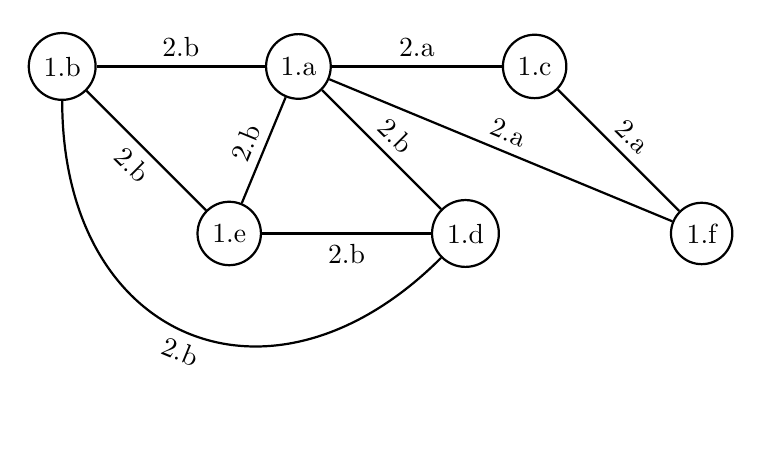
\begin{tikzpicture}[thick, main/.style = {draw, circle}, node distance = 30mm]
    \node[main] (1) {1.a};
    \node[main] (2) [left of=1] {1.b};
    \node[main] (3) [right of=1] {1.c};
    \node[main] (4) [below right of=1] {1.d};
    \node[main] (5) [below right of=2] {1.e};
    \node[main] (6) [below right of=3] {1.f};
    \draw (1) to node[midway, above] {2.b} (2);
    \draw (1) to node[midway, above] {2.a} (3);
    \draw (1) to node[midway, above, sloped] {2.b} (4);
    \draw (1) to node[midway, above, sloped] {2.b} (5);
    \draw (1) to node[midway, above, sloped] {2.a} (6);
    \draw (2) to [out=270, in=225, looseness=1.5] node[midway, below, sloped] {2.b} (4);
    \draw (2) to node[midway, below, sloped] {2.b} (5);
    \draw (3) to node[midway, above, sloped] {2.a} (6);
    \draw (4) to node[midway, below, sloped] {2.b} (5);
\end{tikzpicture}
\subsection{Objetos são filmes}
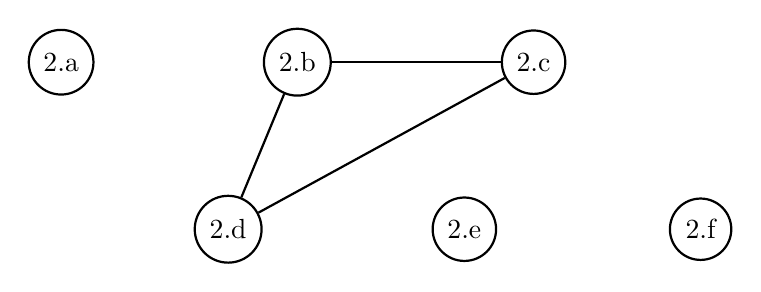
\begin{tikzpicture}[thick, main/.style = {draw, circle}, node distance = 30mm]
    \node[main] (1) {2.a};
    \node[main] (2) [right of=1] {2.b};
    \node[main] (3) [right of=2] {2.c};
    \node[main] (4) [below right of=1] {2.d};
    \node[main] (5) [below right of=2] {2.e};
    \node[main] (6) [below right of=3] {2.f};
    \draw (2) to (3);
    \draw (2) to (4);
    \draw (3) to (4);
\end{tikzpicture}
\subsection{Objetos são filmes e atores}
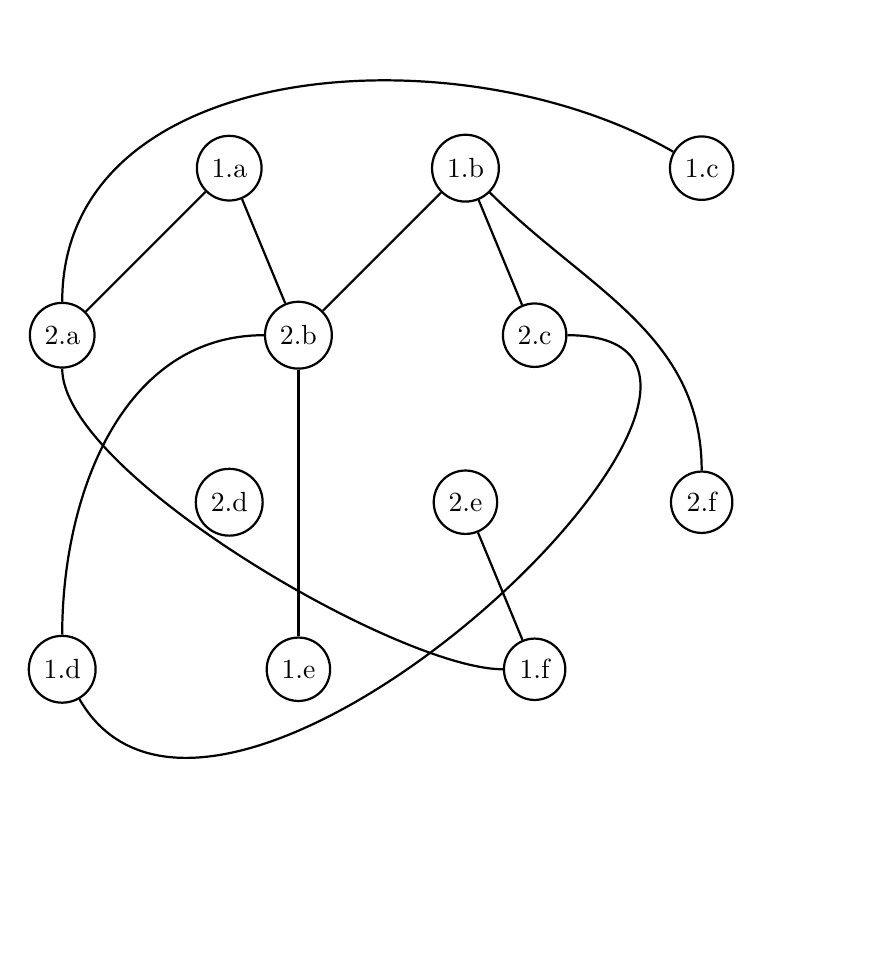
\begin{tikzpicture}[thick, main/.style = {draw, circle}, node distance = 30mm]
    \node[main](1) {1.a};
    \node[main](2) [right of=1] {1.b};
    \node[main](3) [right of=2] {1.c};
    \node[main](4) [below left of=1] {2.a};
    \node[main](5) [right of=4] {2.b};
    \node[main](6) [right of=5] {2.c};
    \node[main](7) [below right of=4] {2.d};
    \node[main](8) [right of=7] {2.e};
    \node[main](9) [right of=8] {2.f};
    \node[main](10) [below left of=7] {1.d};
    \node[main](11) [right of=10] {1.e};
    \node[main](12) [right of=11] {1.f};
    \draw (1) to (4);
    \draw (1) to (5);
    \draw (2) to (5);
    \draw (2) to (6);
    \draw (2) to [out=315, in=90](9);
    \draw (3) to [out=150, in=90](4);
    \draw (10) to [out=90, in=180](5);
    \draw (10) to [out=300, in=0, looseness=1.2](6);
    \draw (11) to (5);
    \draw (12) to [out=180, in=270, looseness=0.5](4);
    \draw (12) to (8);
\end{tikzpicture}

\newpage
\section{Questão 2}
\subsection{Maior Clique do Grafo}
\subsubsection{Grafo 1.1}
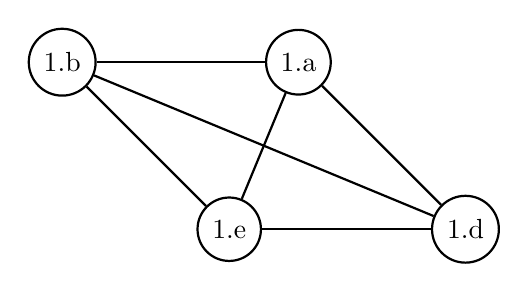
\begin{tikzpicture}[thick, main/.style = {draw, circle}, node distance = 30mm]
    \node[main](1) {1.b};
    \node[main](2) [right of=1]{1.a};
    \node[main](3) [below right of=1] {1.e};
    \node[main](4) [right of=3]{1.d};
    \draw (1) to (2);
    \draw (1) to (3);
    \draw (1) to (4);
    \draw (2) to (3);
    \draw (2) to (4);
    \draw (3) to (4);
\end{tikzpicture}
\subsubsection{Grafo 1.2}
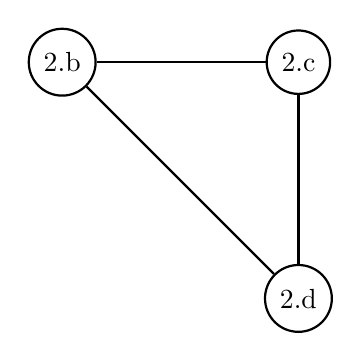
\begin{tikzpicture}[thick, main/.style = {draw, circle}, node distance = 30mm]
    \node[main](1) {2.b};
    \node[main](2) [right of=1]{2.c};
    \node[main](3) [below of=2]{2.d};
    \draw (1) to (2);
    \draw (2) to (3);
    \draw (1) to (3);
\end{tikzpicture}
\subsubsection{Grafo 1.3}
Esse grafo possui apenas cliques triviais de apenas uma aresta, podendo ser exemplificado por:
\smallbreak
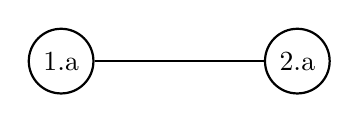
\begin{tikzpicture}[thick, main/.style = {draw, circle}, node distance = 30mm]
    \node[main](1) {1.a};
    \node[main](2) [right of=1]{2.a};
    \draw (1) to (2);
\end{tikzpicture}
\subsection{Diâmetro do Grafo}
\subsubsection{Grafo 1.1}
O diâmetro desse grafo é 2.
\subsubsection{Grafo 1.2}
O diâmetro desse grafo é 1.
\subsubsection{Grafo 1.3}
O diâmetro desse grafo é 5.
\subsection{Existência de Ciclo Hamiltoniano}
\subsubsection{Grafo 1.1}
Não existe um ciclo Hamiltoniano nesse grafo, verificado por inspeção visual.
\subsubsection{Grafo 1.2}
Não existe um ciclo Hamiltoniano nesse grafo, verificado por inspeção visual.
\subsubsection{Grafo 1.3}
Não existe um ciclo Hamiltoniano nesse grafo, verificado por inspeção visual.
\subsection{Existência de Ciclo Euleriano}
\subsubsection{Grafo 1.1}
Não existe um ciclo Euleriano nesse grafo, verificado por inspeção visual.
\subsubsection{Grafo 1.2}
Não existe um ciclo Euleriano nesse grafo, verificado por inspeção visual.
\subsubsection{Grafo 1.3}
Não existe um ciclo Euleriano nesse grafo, verificado por inspeção visual.
\subsection{Bipartição do Grafo}
\subsubsection{Grafo 1.1}
Não existem conjuntos {$V_1$} e {$V_2$} tais que a intersecção entre eles seja o conjunto vazio.
\subsubsection{Grafo 1.2}
Não existem conjuntos {$V_1$} e {$V_2$} tais que a intersecção entre eles seja o conjunto vazio.
\subsubsection{Grafo 1.3}
Por definição este grafo é bipartido, já que relaciona dois tipos diferentes de dados (atores e filmes).
\newpage
\section{Questão 3}
Os atores escolhidos foram os mesmos presentes na Questão 1:
\begin{enumerate}
    \item Wagner Moura - 2
    \item Morena Baccarin - 2
    \item Alice Braga - 2

O maior número (finito) que encontrei foi para o ator Leandro Mazzini, principal de uma série B brasileira. Passando por filmes como "Os homens são de Marte e é pra lá que eu vou" o número de Bacon do ator é 4.
\end{enumerate}

\section{Questão 4}
Meu número de Erdős é 4, seguindo o caminho:

Marinho, K. {$\leftarrow$} Figueiredo, Daniel Ratton {$\leftarrow$} Reed, Bruce A. {$\leftarrow$} Alon, Noga {$\leftarrow$} Erdős, Paul

\section{Questão 5}
\subsection{Caminho entre UFRJ e MIT}
\begin{enumerate}
    \item www.ufrj.br
    \item https://internacional.ufrj.br/
    \item https://internacional.ufrj.br/pesquisaacordos/
    \item https://www.nyu.edu/
    \item https://x.com/nyuniversity
    \item https://x.com/i/connect\_people?user\_id=28421825 (Página de sugestões de follow do X)
    \item https://x.com/MIT
    \item http://socialmediahub.mit.edu/
    \item https://web.mit.edu/
    O comprimento total do caminho é 8.
\end{enumerate}
\subsection{Caminho alternativo entre UFRJ e MIT}
\begin{enumerate}
    \item https://ufrj.br/
    \item https://acessibilidade.ufrj.br/
    \item https://www.gov.br/pt-br
    \item https://creativecommons.org/licenses/by-nd/3.0/deed.en
    \item https://creativecommons.org/share-your-work/cclicenses/
    \item https://creativecommons.org/faq/
    \item https://ocw.mit.edu/
    \item https://openlearning.mit.edu/
    \item https://openlearning.mit.edu/accessibility
    \item https://accessibility.mit.edu/
    \item https://web.mit.edu/
    O comprimento total do caminho é 10.
\subsection{Como encontrar o menor cmainoh possível}
Uma forma simples que acredito cumprir o trabalho, apesar de ser extrememante não eficiente, é "inundar" todos os possíveis caminho entre dois vértices presentes no grafo e após isso selecionar o que possuir menor valor. Essa abordagem no entanto poderia ser muito demorada, e sem uma inteligência maior para o algoritmo ele acabaria repetindo muitos caminhos ou não chegando a lugar algum em algumas ocasiões
\end{enumerate}
\end{document}
